\chapter{Analýza}
Následující kapitola se zabývá analýzou existujících řešení, popisuje funkční a~nefunkční požadavky na~novou aplikaci a~v~neposlední řadě obsahuje jednotlivé případy užití, které představují detailnější specifikaci dříve uvedených funkčních požadavků.

\section{Existující řešení}
Následující podkapitola je věnována již existujícím informačním systémům, které by měly usnadnit sportovním klubům a~skupinám administrativní činnost. V~současné době jich na~trhu existuje již~poměrně velké množství, a~proto se zaměřím pouze na~ty, které mi přišly nejrozšířenější nebo~nějakým způsobem zajímavé. V~následujících sekcích budou přiblížena dvě řešení z~komerční sféry, jeden bezplatný systém a~také bude podrobněji představena aplikace, která je v~současné době využívána klubem KOB~Ústí nad~Orlicí.

Několik systémů, které mají řešit podobné problémy, vzniklo v~minulosti i~v~rámci závěrečných prací na~různých českých univerzitách. Pro~kompletnost mohu například zmínit práce \cite{fimuni2021, fitcvut2016, fisvse2013}, avšak jejich obsah zde nebudu detailněji rozebírat.

\subsection{KUOris}
\label{section:kuoris}
Klub orientačního běhu~Ústí nad~Orlicí nyní využívá pro~přihlašování na~závody webovou aplikaci KUOris. Tento systém vznikl v~roce 2016 jako nástupce řešení, které bylo založené na~open source systému phpBB, jenž je nejčastěji využíván pro~tvorbu diskuzního fóra \cite{phpbb}. V~průběhu let byl drobně upravován, avšak z~důvodu špatného návrhu není možné do~systému KUOris jednoduše přidávat nové funkcionality.

Systém v aktuálním stavu podporuje přidávání a~následné spravování událostí. Při~vytváření události se členům klubu, kteří si tuto funkcionalitu povolili, zasílá informační e-mail se základními informacemi o~dané akci. Na~jednotlivé události se členové klubu mohou přihlašovat a~mohou k~nim psát komentáře.

Mezi~největší nedostatky aplikace KUOris se řadí zastaralé uživatelské rozhraní a~chybějící automatizace. V~dnešní době, kdy na~web přistupuje více lidí z~mobilních zařízení než~z~počítačů~\cite{deviceusage}, by mělo být uživatelské rozhraní jistě responzivní. Další již zmíněný nedostatek spatřuji u nevyužité možnosti automatizace. IS~ORIS nabízí API, jež je detailněji popsané v sekci \ref{implementation:oris-api}, pro~získávání informací o~závodech a~i~pro~přihlašování na~jednotlivé akce. V současném systému této možnosti není využíváno a~všechny úkony tedy musí administrátor provádět ručně.

\begin{description}
	\item[Nevýhody:] složitá rozšiřitelnost, neresponzivní UI, absence propojení s~IS ORIS
\end{description}

\subsection{KIS~–~Klubový Informační Systém}
KIS je komplexní klubový informační systém, který je díky svým pokročilým funkcionalitám využíván i~největšími sportovními subjekty v~České republice. Mezi uživatele systému se totiž například řadí Český svaz ledního hokeje, Fotbalová asociace České republiky, Český olympijský výbor a~další velké fotbalové a~hokejové kluby. \cite{esports, ceskyhokej}

Mezi klíčové funkčnosti systému se řadí podpora pro~pořádání klubových akcí, správa plateb, evidence dokumentů, zobrazování statistik, kalendář a~mnoho dalších funkcí. K~systému je možné přistupovat i~přes~mobilní aplikaci, která je dostupná pro~zařízení s~operačním systém iOS a~Android. Jedná se o~komerční systém, dle ceníku se cena skládá z~jednorázového počátečního poplatku 9~900~Kč bez~DPH a~následného měsíčního poplatku 300~Kč bez~DPH za~technickou správu. \cite{esports}

\begin{description}
	\item[Výhody:] komplexní klubový systém s~pokročilými funkcemi a~mobilní aplikací
	\item[Nevýhody:] nákladnost (jednorázový a~následné měsíční poplatky), absence propojení s~IS ORIS
\end{description}

\subsection{Sportes~–~Český sportovní evidenční systém}
Jedná se o~další komplexní systém pro~sportovní kluby, ke~kterému je opět možné přistupovat jak z~webového prohlížeče, tak i~z~mobilní aplikace. Obsahuje podobné funkcionality jako systém KIS, tj.~správu událostí, evidenci členské základny, docházky a~plateb. Pro~menší sportovní kluby však pravděpodobně bude překážkou pro~jeho využívání uvedená cena, neboť za~variantu pro~maximálně 100~členů je stanovena na~12~000~Kč bez~DPH ročně. \cite{sportes}

\begin{description}
	\item[Výhody:] systém pro kompletní správu sportovního klubu s vlastní mobilní aplikací
	\item[Nevýhody:] nákladnost (12~000~Kč za~rok bez~DPH), absence propojení s~IS ORIS
\end{description}

\subsection{Týmuj}
Týmuj je online služba, která byla do~ostrého provozu spuštěna v~květnu roku 2008. Od~té doby v ní bylo vytvořeno přes~30~000~týmů a~svůj účet si vytvořilo přes~250~000~sportovců. Služba Týmuj je od~svého vzniku neustále vylepšována a~v~roce 2017 byly spuštěny i~mobilní aplikace pro~operační systémy iOS a~Android.

Týmuj umožňuje vytvářet a~spravovat události, evidovat docházku u~jednotlivých událostí, posílat zprávy do~týmového chatu a~k~jednotlivým akcím, evidenci týmových plateb, sdílení fotografií a~mnoho dalších věcí. V~rámci týmu mají jednotliví členové jednu ze~tří rolí (majitel, správce nebo~hráč) a~na~základě přidělené role mají odpovídající práva.

Popularitu tohoto online nástroje dokazuje fakt, že jen za~poslední rok bylo přes~Týmuj zorganizováno přes~300~000~událostí. Takový počet akcí bude jistě z~nemalé části způsoben tím, že využívání Týmuj není zpoplatněno a~že~taktéž neexistuje omezení na~maximální počet členů týmu. \cite{tymuj}

\begin{description}
	\item[Výhody:] užívání není zpoplatněno, obsahuje mnoho funkcí, existuje webová i mobilní aplikace
	\item[Nevýhody:] absence propojení s~IS ORIS
\end{description}
\newpage

\section{Funkční požadavky}
Funkční požadavky popisují požadované funkcionality systému. Mohou například specifikovat, jakým způsobem bude uživatel moci pracovat se systémem, jaké procesy by měl systém podporovat a~jaké budou vstupy a~výstupy těchto procesů. \cite{requirements}

\begin{enumerate}[label=\textcolor{decoration}{\textbf{F\arabic*}}, leftmargin=6mm]
	\myItem{evidence a~správa uživatelů}
	Systém bude umožňovat registraci nových uživatelů, neregistrovaný uživatel nemá přístup do~systému. Při~registraci bude nutno zadat minimálně registrační číslo, e-mailovou adresu, heslo a~jméno a~příjmení člena klubu. Právě pomocí registračního čísla a~zadaného hesla bude následně uživatel přistupovat do~systému.

	Kromě těchto základních údajů bude mít administrátor možnost uživateli nastavovat a~upravovat stav osobního konta, typ členství (aktivní nebo~pasivní) a~roli (viz~sekce \ref{section:role}). Uživatele musí být možno anonymizovat kvůli GDPR.

	\myItem{evidence a~správa závodů a~tréninků\label{f:events}}
	Dále systém bude umožňovat evidenci a~správu tréninků a~závodů (událostí). Konkrétně je potřeba mít možnost u~každé události evidovat:
	\begin{itemize}
		\item název
		\item typ události (trénink nebo~závod)
		\item datum a~čas události (kdy událost začíná)
		\item místo konání
		\item pořadatel
		\item datum a~čas uzávěrky přihlášek
		\item disciplínu
		\item vypsané kategorie
		\item další informace
		\item v~případě závodu bude možné dále evidovat:
		\begin{itemize}
			\item typ závodu
			\item webovou stránku
		\end{itemize}
		\item u~tréninku bude možné oproti závodu naopak evidovat maximální kapacitu
	\end{itemize}

	Samotné zadání události do~systému bude umožněno ručním vyplněním všech požadovaných údajů nebo~automatickým importem z~informačního systému Českého svazu orientačních sportů pomocí unikátního identifikátoru závodu.

	Na~hlavní stránce systému by se měly zobrazovat závody a tréninky s~nejbližší uzávěrkou přihlášek. V~zadaných trénincích a~závodech bude možné vyhledávat a~filtrovat a~zadanou událost musí být možno zrušit bez~odstraňování ze~systému. Taková událost bude následně od~nezrušených událostí vizuálně odlišena a~nebude možné se na~ni dále přihlašovat.

	\myItem{přihlašování na~závody a~tréninky}
	Na~událost evidovanou v~systému se mohou registrovaní uživatelé přihlásit, pokud dosud neproběhla uzávěrka přihlášek. Při~přihlášení si uživatelé musí navíc vybrat jednu z~nabízených kategorií, do~které se chtějí přihlásit, a~mohou volitelně sdělit, zdali mají možnost jet vlastním autem a~svést s~sebou i~další členy klubu. Svou účast mohou uživatelé do~konce uzávěrky přihlášek také odřeknout.

	\myItem{synchronizace přihlášek}
	Po~skončení termínu přihlášek bude mít trenér možnost odeslat všechny evidované přihlášky do~IS~ORIS přes~jeho API. Tato možnost bude ze~zřejmých důvodů dostupná pouze pro~závody, které jsou v~IS~ORIS evidované.

	\myItem{e-mailová upozornění --- TODO: asi odebrat}
	Systém bude umožňovat při~přidávání události odeslat informační e-mail se základními informacemi o~dané události. E-mail bude odeslán pouze těm registrovaným uživatelům, kteří si ve~svém nastavení povolili zasílání e-mailových upozornění.

	\myItem{oznámení}
	Trenéři a~administrátoři systému budou mít možnost vytvořit oznámení, která se budou zobrazovat na~hlavní stránce systému.

	\myItem{komentáře}
	Komentáře mohou psát registrovaní uživatelé ke~všem tréninkům a~závodům. Nejnovější komentáře by se měly zobrazovat (včetně informace kam byly napsány) na~hlavní stránce systému.
\end{enumerate}

\subsection{Role}
\label{section:role}
Každému uživateli bude náležet právě jedna z~následujících uživatelských rolí:
\begin{itemize}
	\item registrovaný uživatel
	\begin{itemize}
		\item základní uživatelská role, která nemá žádná speciální oprávnění
		\item výčet akcí, které může registrovaný uživatel vykonávat:
		\begin{itemize}
			\item přihlašovat a~odhlašovat se z~tréninků a~závodů
			\item psát komentáře k~jednotlivým tréninkům a~závodům a~následně je i~upravovat
			\item měnit svou e-mailovou adresu a~heslo pro~přihlášení do~systému
			\item nastavit si zasílání e-mailových upozornění na~nově přidané události do~systému --- TODO
		\end{itemize}
	\end{itemize}
	\item trenér
	\begin{itemize}
		\item role, která náleží trenérům působícím v~klubu
		\item oproti roli registrovaný uživatel má právo:
		\begin{itemize}
			\item přidávat a~následně spravovat tréninky a~závody
			\item odeslat evidované přihlášky do~IS~ORIS
			\item psát a~upravovat svá oznámení
		\end{itemize}
	\end{itemize}
	\item administrátor
	\begin{itemize}
		\item má kompletní přístup ke~všem funkcionalitám systému
		\item oproti uživatelům s~rolí trenér může navíc:
		\begin{itemize}
			\item upravovat a~mazat veškeré komentáře a oznámení
			\item spravovat uživatele
			\item odhlašovat a~přihlašovat uživatele na~tréninky a~závody (i~po~termínu přihlášek)
			\item odebírat a~přidávat informaci o~možnosti vzít auto (i~po~termínu přihlášek)
		\end{itemize}
	\end{itemize}
\end{itemize}

\section{Nefunkční požadavky}
Nefunkční požadavky se na~rozdíl od~funkčních požadavků zabývají vlastnostmi a~omezeními daného systému. Mohou se mezi~nimi objevit požadavky, které budou podstatné jak~pro~samotné uživatele systému, jako například doba odezvy, zabezpečení systému, způsob zobrazování na~mobilních zařízeních, tak zde mohou být uvedeny i~požadavky techničtějšího charakteru, jako~například použití konkrétních technologií nebo~možnost snadné rozšiřitelnosti systému. \cite{requirements}

\begin{enumerate}[label=\textcolor{decoration}{\textbf{N\arabic*}}]
	\myItem{responzivita}
	Webová aplikace bude přizpůsobovat svůj vzhled na~základě rozlišení klientského zařízení.

	\myItem{lokalizace}
	Aplikace by měla být připravena na~přeložení do~dalších jazyků.

	\myItem{technologie}
	Aplikace bude napsána v~programovacím jazyce PHP ve~frameworku Symfony.

	\myItem{zabezpečení}
	Komunikace s~aplikací bude probíhat pouze přes~zabezpečený protokol HTTPS.

	\myItem{rozšiřitelnost a~modifikovatelnost}
	Aplikace by měla být snadno rozšiřitelná a~modifikovatelná. Její využití by tedy nemělo být limitováno pouze na~kluby orientačního běhu, ale své uplatnění by měla nalézt i~u~sportovních organizací zabývajících se jiným sportem.

	\myItem{výkon~a dostupnost}
	Aplikace bude schopná v~jednu chvíli obsluhovat jednotky až~nižší desítky uživatelů s~odezvou v~řádu sekund.
\end{enumerate}

\section{Případy užití}
Tato podkapitola se věnuje jednotlivým případům užití, které představují detailnější specifikaci funkčních požadavků. Případy užití poté mohou posloužit jako základ pro~tvorbu uživatelské dokumentace a~také mohou být podkladem pro~tvorbu akceptačních testů. \cite{usecases}

\subsection{Aktéři}
Aktérem nebo~účastníkem nazýváme osobu (případně její roli), která bude pracovat se systémem. V~naší aplikaci uvažujeme celkem čtyři různé aktéry~–~přihlášeného a~nepřihlášeného uživatele, administrátora a~trenéra. Vztahy mezi těmito aktéry jsou popsány v~následujícím textu a~jsou znázorněny na~obrázku \ref{figure:actors}.
\begin{description}
	\item[Nepřihlášený uživatel]\hfill\newline
	Nepřihlášený uživatel má přístup pouze k~přihlášení a~registraci. Po~provedení jedné z~těchto akcí se stane přihlášeným uživatelem.
	\item[Přihlášený uživatel]\hfill\newline
	Přihlášený uživatel má práva, která byla již dříve popsána v~sekci \ref{section:role} u~role registrovaný uživatel. Jelikož je uživatel již přihlášený do~systému, tak nemá přístup k~přihlašovací stránce a~k~registraci.
	\item[Trenér]\hfill\newline
	Práva trenéra vycházejí z~práv přihlášeného uživatele a~navíc zahrnují práva na~správu závodů a~tréninků. Podrobný popis práv lze nalézt v~sekci \ref{section:role} u~role trenér.
	\item[Administrátor]\hfill\newline
	Administrátor má přístup ke~všem funkcionalitám systému. Jeho práva jsou popsána v~sekci \ref{section:role} u~role administrátor.
\end{description}

\begin{figure}[h]
	\caption{Aktéři}
	\label{figure:actors}
	\centering
	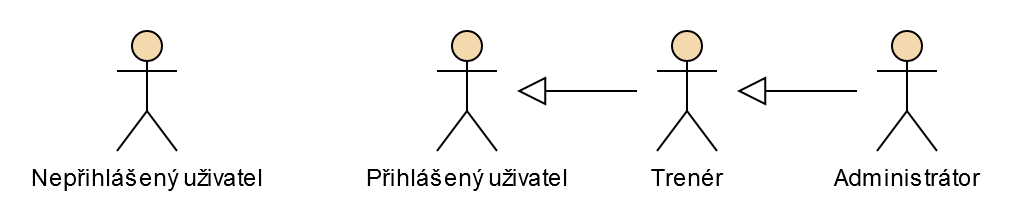
\includegraphics[width=0.9\textwidth]{images/actors}
\end{figure}

\subsection{Případy užití}
\begin{enumerate}[label=\textcolor{decoration}{\textbf{UC\arabic*}}, leftmargin=1cm, align=left, labelwidth=8mm]

	\myItem{registrace}
	Před~prvním přístupem do~systému se musí člen klubu zaregistrovat. 
	\begin{enumerateNumbers}
		\item Nepřihlášený uživatel klikne na~položku \emph{Registrace} v~hlavní nabídce.
		\item Pro~úspěšné dokončení registrace musí vyplnit svou e-mailou adresu, heslo, jméno a~příjmení a~kliknout na~tlačítko \emph{Registrovat}.
		\item Registraci musí následně schválit některý z~administrátorů a~poté se již nepřihlášený uživatel může pomocí zadané e-mailové adresy a~hesla přihlásit do~systému.
	\end{enumerateNumbers}

	\myItem{přihlášení a~odhlášení z~aplikace}
	Nepřihlášený uživatel bude při~pokusu o~přístup do~systému vyzván k~přihlášení.
	\begin{enumerateNumbers}
		\item Nepřihlášený uživatel zadá svou e-mailovou adresu a~heslo a~klikne na~tlačítko \emph{Přihlásit}.
		\item Pokud přihlášení proběhlo úspěšně, bude uživatel přesměrován na~hlavní stránku aplikace nebo~na~stránku, na~kterou se snažil před~přihlášením přistoupit.
		\item Přihlášený uživatel má naopak možnost se ze~systému odhlásit kliknutím na~položku \emph{Odhlásit} v~hlavní nabídce.
	\end{enumerateNumbers}
	\newpage

	\myItem{zobrazení seznamu událostí\label{uc:listevents}}
	Tento případ užití popisuje proces zobrazení seznamu událostí evidovaných v~systému.
	\begin{enumerateNumbers}
		\item Přihlášený uživatel klikne na~položku \emph{Události} v~hlavní nabídce
		\item Ve~výchozím nastavení se zobrazují všechny nadcházející události, avšak upravením filtru v~horní části stránky lze zobrazit i~minulé události nebo~provést filtraci na~základě typu události, případně na~základě typu závodu.
		\item Na~jedné stránce se vždy zobrazuje maximální 25~událostí, další události je možné zobrazit přejitím na~následující (předchozí) stránku.
	\end{enumerateNumbers}

	\myItem{zobrazení detailních informací o~události\label{uc:eventdetail}}
	V~seznamu událostí jsou zobrazovány pouze základní informace o~událostech, pro~zobrazení detailních informací je nezbytné přejít na~samostatnou stránku.
	\begin{enumerateNumbers}
		\item Přihlášený uživatel se může prokliknout na~stránku s~informacemi o~události z(e):
		\begin{enumerate}[label=\textcolor{decoration}{\textbf{\alph*.}}]
			\item seznamu událostí (viz~\ref{uc:listevents}).
			\item hlavní stránky, kde se zobrazuje 5~událostí, u~kterých nejdříve končí uzávěrka přihlášek, a~5~nejbližších událostí, na~které je uživatel přihlášený.
		\end{enumerate}
		\item Přechod na~stránku se~všemi evidovanými informacemi o~události (viz~\ref{f:events}) proběhne po~kliknutí na~název události v~jednom ze~seznamů uvedených výše.
	\end{enumerateNumbers}

	\myItem{přihlášení na~událost}
	Přihlášení na~událost je možné provést pouze pokud událost nebyla zrušena, neproběhla uzávěrka přihlášek a~pokud již není daný uživatel na~danou událost přihlášený.
	\begin{enumerateNumbers}
		\item Přihlášený uživatel přejde na~stránku s~detailními informacemi o~události (viz~\ref{uc:eventdetail}).
		\item Uživatel vybere jednu z~nabízených kategorií a~volitelně sdělí, zda má možnost jet vlastním autem a~svézt s~sebou i~další členy klubu.
		\item Účast na~události potvrdí uživatel kliknutím na~tlačítko \emph{Přihlásit}.
	\end{enumerateNumbers}

	\myItem{odhlášení z~události}
	Odhlášení z~události je možné provést pouze pokud nebyla událost zrušena, neproběhla uzávěrka přihlášek a~pokud je daný uživatel na~danou událost přihlášený.
	\begin{enumerateNumbers}
		\item Přihlášený uživatel přejde na~stránku s~detailními informacemi o~události (viz~\ref{uc:eventdetail}).
		\item Účast na~události uživatel odřekne kliknutím na~tlačítko \emph{Odhlásit}.
	\end{enumerateNumbers}

	\myItem{přidání a~úprava komentáře}
	Tento případ užití popisuje přidání a~následnou úpravu komentáře u~konkrétní události.
	\begin{enumerateNumbers}
		\item Přihlášený uživatel přejde na~stránku s~detailními informacemi o~události (viz~\ref{uc:eventdetail}).
		\item Po~napsání komentáře do~textového pole klikne na~tlačítko \emph{Přidat komentář}.
		\item Své komentáře má uživatel možnost upravit kliknutím na~ikonku pro~úpravu vedle konkrétního komentáře. To načte napsaný komentář do~textového pole a~po~jeho úpravě dojde k~uložení kliknutím na~tlačítko \emph{Upravit komentář}.
	\end{enumerateNumbers}

	\myItem{úprava osobních údajů a~preferencí}
	Přihlášený uživatel si může změnit svou e-mailovou adresu, heslo a~povolit (zakázat) zasílání informačních e-mailů.
	\begin{enumerateNumbers}
		\item Přihlášený uživatel klikne na~položku \emph{Nastavení} v~hlavní nabídce.
		\item Po~upravení požadovaných údajů a~preferencí klikne na~tlačítko \emph{Uložit změny}.
	\end{enumerateNumbers}

	\myItem{přidání události}
	Tento případ užití popisuje přidání nové události do~systému.
	\begin{enumerateNumbers}
		\item Trenér klikne na~položku \emph{Administrace} v~hlavní nabídce a~následně vybere možnost \emph{Vytvořit novou událost}.
		\item Pokud je přidávaná událost již evidovaná v~IS~ORIS, může uživatel zadat ORIS~ID události a~většina požadovaných informací se automaticky předvyplní.
		\item Po~(do)vyplnění požadovaných informací se událost přidá do~systému kliknutím na~tlačítko \emph{Přidat novou událost}.
	\end{enumerateNumbers}

	\myItem{úprava události}
	Tento případ užití popisuje proces upravení události již evidované v~systému.
	\begin{enumerateNumbers}
		\item Trenér klikne na~položku \emph{Administrace} v~hlavní nabídce a~následně vybere ze~seznamu událost, kterou si přeje upravit.
		\item Po~upravení požadovaných informací klikne na~tlačítko \emph{Uložit změny}.
	\end{enumerateNumbers}

	\myItem{synchronizace přihlášek}
	Role trenér v~systému sama o~sobě nestačí pro~odeslání přihlášek do~IS~ORIS. Je zapotřebí, aby uživatel měl také zřízený účet v~IS~ORIS a~měl práva na~přihlašování závodníků klubu.
	\begin{enumerateNumbers}
		\item Trenér klikne na~položku \emph{Administrace} v~hlavní nabídce a~následně vybere možnost \emph{Synchronizace přihlášek}.
		\item Na~zobrazené stránce vybere požadovanou událost a~zadá přístupové údaje do~IS~ORIS.
		\item Přihlášky evidované u~dané události budou odeslány po~kliknutí na~tlačítko \emph{Synchronizovat přihlášky}.
	\end{enumerateNumbers}

	\myItem{vytvoření, úprava a smazání oznámení}
	Tento případ užití popisuje vytvoření, úpravu a~smazání oznámení.
	\begin{enumerateNumbers}
		\item Trenér na~hlavní stránce klikne na~ikonku pro~přidání nového oznámení nebo~na~ikonku pro~upravení již~existujícího oznámení.
		\item Po~vyplnění (upravení) požadovaných informací klikne na~tlačítko \emph{Uložit oznámení}.
		\item Pro~smazání oznámení klikne trenér na~ikonku koše vedle odpovídajícího oznámení a~v~následně zobrazeném dialogu smazání potvrdí.
	\end{enumerateNumbers}

	\myItem{úprava a anonymizace uživatele}
	Funkce anonymizace uživatele přenastaví uživatelovo jméno na~\emph{Anonymní uživatel} a~smaže všechny jeho údaje (registrační číslo, stav osobního konta, typ členství, e-mail a~heslo). Tímto je uživateli znemožněno přihlášení do~aplikace.
	\begin{enumerateNumbers}
		\item Administrátor klikne na~položku \emph{Administrace} v~hlavní nabídce a~následně vybere ze~seznamu uživatele, kterého si přeje upravit.
		\item Po~upravení požadovaných informací klikne na~tlačítko \emph{Uložit změny}.
		\item Anonymizaci uživatele lze provést kliknutím na~tlačítko \emph{Anonymizovat uživatele}.
	\end{enumerateNumbers}

\end{enumerate}
\newpage

\subsection{Pokrytí funkčních požadavků v případech užití}
V~tabulce \ref{table:use-cases} je zachyceno pokrytí funkčních požadavků v~jednotlivých případech užití. Symbol~\Checkmark říká, že příslušný funkční požadavek je součástí daného případu užití.

\begin{table}[h]
	\centering
	\caption{\label{table:use-cases}Mapování funkčních požadavků na~případy užití}
	\begin{tabularx}{0.95\textwidth}{|C||C|C|C|C|C|C|C|}
		\hline
			 & F1 & F2 & F3 & F4 & F5 & F6 & F7 				\\ \hline\hline
		UC1  & \Checkmark &    &    &    &    &    &    		\\ \hline
		UC2  & \Checkmark &    &    &    &    &    &    		\\ \hline
		UC3  &    & \Checkmark &    &    &    &    &    		\\ \hline
		UC4  &    & \Checkmark &    &    &    &    &    		\\ \hline
		UC5  &    &    & \Checkmark &    &    &    &    		\\ \hline
		UC6  &    &    & \Checkmark &    &    &    &    		\\ \hline
		UC7  &    &    &    &    &    &    & \Checkmark 		\\ \hline
		UC8  & \Checkmark &    &    &    & \Checkmark &    &	\\ \hline
		UC9  &    & \Checkmark &    &    & \Checkmark &    &	\\ \hline
		UC10 &    & \Checkmark &    &    &    &    &    		\\ \hline
		UC11 &    &    &    & \Checkmark &    &    &    		\\ \hline
		UC12 &    &    &    &    &    & \Checkmark &    		\\ \hline
		UC13 & \Checkmark &    &    &    &    &    &    		\\ \hline
	\end{tabularx}
\end{table}

